\documentclass{sigchi}

% Use this command to override the default ACM copyright statement
% (e.g. for preprints).  Consult the conference website for the
% camera-ready copyright statement.

%% EXAMPLE BEGIN -- HOW TO OVERRIDE THE DEFAULT COPYRIGHT STRIP -- (July 22, 2013 - Paul Baumann)
% \toappear{Permission to make digital or hard copies of all or part of this work for personal or classroom use is      granted without fee provided that copies are not made or distributed for profit or commercial advantage and that copies bear this notice and the full citation on the first page. Copyrights for components of this work owned by others than ACM must be honored. Abstracting with credit is permitted. To copy otherwise, or republish, to post on servers or to redistribute to lists, requires prior specific permission and/or a fee. Request permissions from permissions@acm.org. \\
% {\emph{CHI'14}}, April 26--May 1, 2014, Toronto, Canada. \\
% Copyright \copyright~2014 ACM ISBN/14/04...\$15.00. \\
% DOI string from ACM form confirmation}
%% EXAMPLE END -- HOW TO OVERRIDE THE DEFAULT COPYRIGHT STRIP -- (July 22, 2013 - Paul Baumann)

% Arabic page numbers for submission.  Remove this line to eliminate
% page numbers for the camera ready copy 
% \pagenumbering{arabic}

% Load basic packages
\usepackage{balance}  % to better equalize the last page
\usepackage{graphics} % for EPS, load graphicx instead 
%\usepackage[T1]{fontenc}
\usepackage{txfonts}
\usepackage{times}    % comment if you want LaTeX's default font
\usepackage[pdftex]{hyperref}
% \usepackage{url}      % llt: nicely formatted URLs
\usepackage{color}
\usepackage{textcomp}
\usepackage{booktabs}
\usepackage{ccicons}
%\usepackage{todonotes}
\usepackage{listings}


\usepackage[font=normalsize,labelfont=bf,skip=5pt]{caption}
\usepackage{subcaption}

\usepackage[acronym]{glossaries}

% llt: Define a global style for URLs, rather that the default one
\makeatletter
\def\url@leostyle{%
  \@ifundefined{selectfont}{\def\UrlFont{\sf}}{\def\UrlFont{\small\bf\ttfamily}}}
\makeatother
\urlstyle{leo}

% To make various LaTeX processors do the right thing with page size.
\def\pprw{8.5in}
\def\pprh{11in}
\special{papersize=\pprw,\pprh}
\setlength{\paperwidth}{\pprw}
\setlength{\paperheight}{\pprh}
\setlength{\pdfpagewidth}{\pprw}
\setlength{\pdfpageheight}{\pprh}

% Make sure hyperref comes last of your loaded packages, to give it a
% fighting chance of not being over-written, since its job is to
% redefine many LaTeX commands.
\definecolor{linkColor}{RGB}{6,125,233}
\hypersetup{%
  pdftitle={SIGCHI Conference Proceedings Format},
  pdfauthor={LaTeX},
  pdfkeywords={SIGCHI, proceedings, archival format},
  bookmarksnumbered,
  pdfstartview={FitH},
  colorlinks,
  citecolor=black,
  filecolor=black,
  linkcolor=black,
  urlcolor=linkColor,
  breaklinks=true,
}

\newcommand{\todo}[1]{~\\\\~\textbf{\large{\textcolor{red}{#1}}}\\~\\~\\~\\~}



% define code environment, keeps the listing on the same page, without break
% listing style attributes: https://en.wikibooks.org/wiki/LaTeX/Source_Code_Listings
\lstnewenvironment{code}[1][]%
{\noindent\minipage{\linewidth}\medskip 
	\lstset{
		frame=single,
		numbers=left,
		numbersep=5pt,
		breaklines=true,
		numberstyle=\tiny,
		showstringspaces=false,
		basicstyle=\small\ttfamily,
		captionpos=b,
		#1
	}
}
{\endminipage}

% create a shortcut to typeset table headings
% \newcommand\tabhead[1]{\small\textbf{#1}}


% End of preamble. Here it comes the document.
\begin{document}

\title{From Large Touch Walls to Tablets -- a Responsive Web Framework for Large Multi-Touch Wall Applications}

\numberofauthors{3}
\author{%
  \alignauthor{1st Author Name\\
    \affaddr{Affiliation}\\
    \affaddr{City, Country}\\
    \email{e-mail address}}\\
  \alignauthor{2nd Author Name\\
    \affaddr{Affiliation}\\
    \affaddr{City, Country}\\
    \email{e-mail address}}\\
  \alignauthor{3rd Author Name\\
    \affaddr{Affiliation}\\
    \affaddr{City, Country}\\
    \email{e-mail address}}\\
}

\maketitle

\newacronym{spa}{SPA}{single-page application}
\newacronym{dom}{DOM}{Document Object Model}
\newacronym{rwd}{RWD}{responsive web design}
\newacronym{sp1}{SP1}{sprint planning 1}
\newacronym{sp2}{SP2}{sprint planning 2}
\newacronym{uri}{URI}{uniform resource identifier}


\begin{abstract}
Agile software development is a highly collaborative and communication intensive method in modern software development. One of its characteristics is the usage of large pin boards with cards where the team does the whole project planning. Based on \textit{aWall}, a web based agile collaboration platform using large multi-touch wall systems, we present a responsive web design approach that supports application interaction as a team and as an individual using both the large multi-touch wall system and as well as tablets. Combining these two interaction methods present unique challenges with respect to the UI and the flow of information. We describe \textit{aWall}'s Web UI architecture and implementation for a concrete case study to showcase the collaborative nature of the application with special focus on its responsive design approach, interaction and information dissemination in the multi-device environment.
\end{abstract}

\category{H.5.2.}{Information Interfaces and Presentation (e.g. HCI)}{User Interfaces -- \textit{Interaction styles}}
\category{H.5.3.}{Information Interfaces and Presentation (e.g. HCI)}{Group and Organization Interfaces -- \textit{Computer-supported cooperative work}}
\category{H.5.4.}{Information Interfaces and Presentation (e.g. HCI)}{Hypertext/Hypermedia -- \textit{Architectures}}


\keywords{Collaborative work and interaction; multi-touch; wall; tablets; responsive design; agile; sprint planning 2; web components}

\section{Introduction}
% intro to challenges, motivation
In agile software development physical pin boards, so called task boards, are the main tool for agile project planning. We developed a software-based solution for extra large digital multi-touch wall systems, the \textit{aWall} web application, intended to replace the paper-based pin board.
The system consists of two distinct device types: The wall as a direct replacement for the pin board (see Figure~\ref{fig:awall}) and tablets for more input-oriented tasks.

\begin{figure}[h]
	\centering
	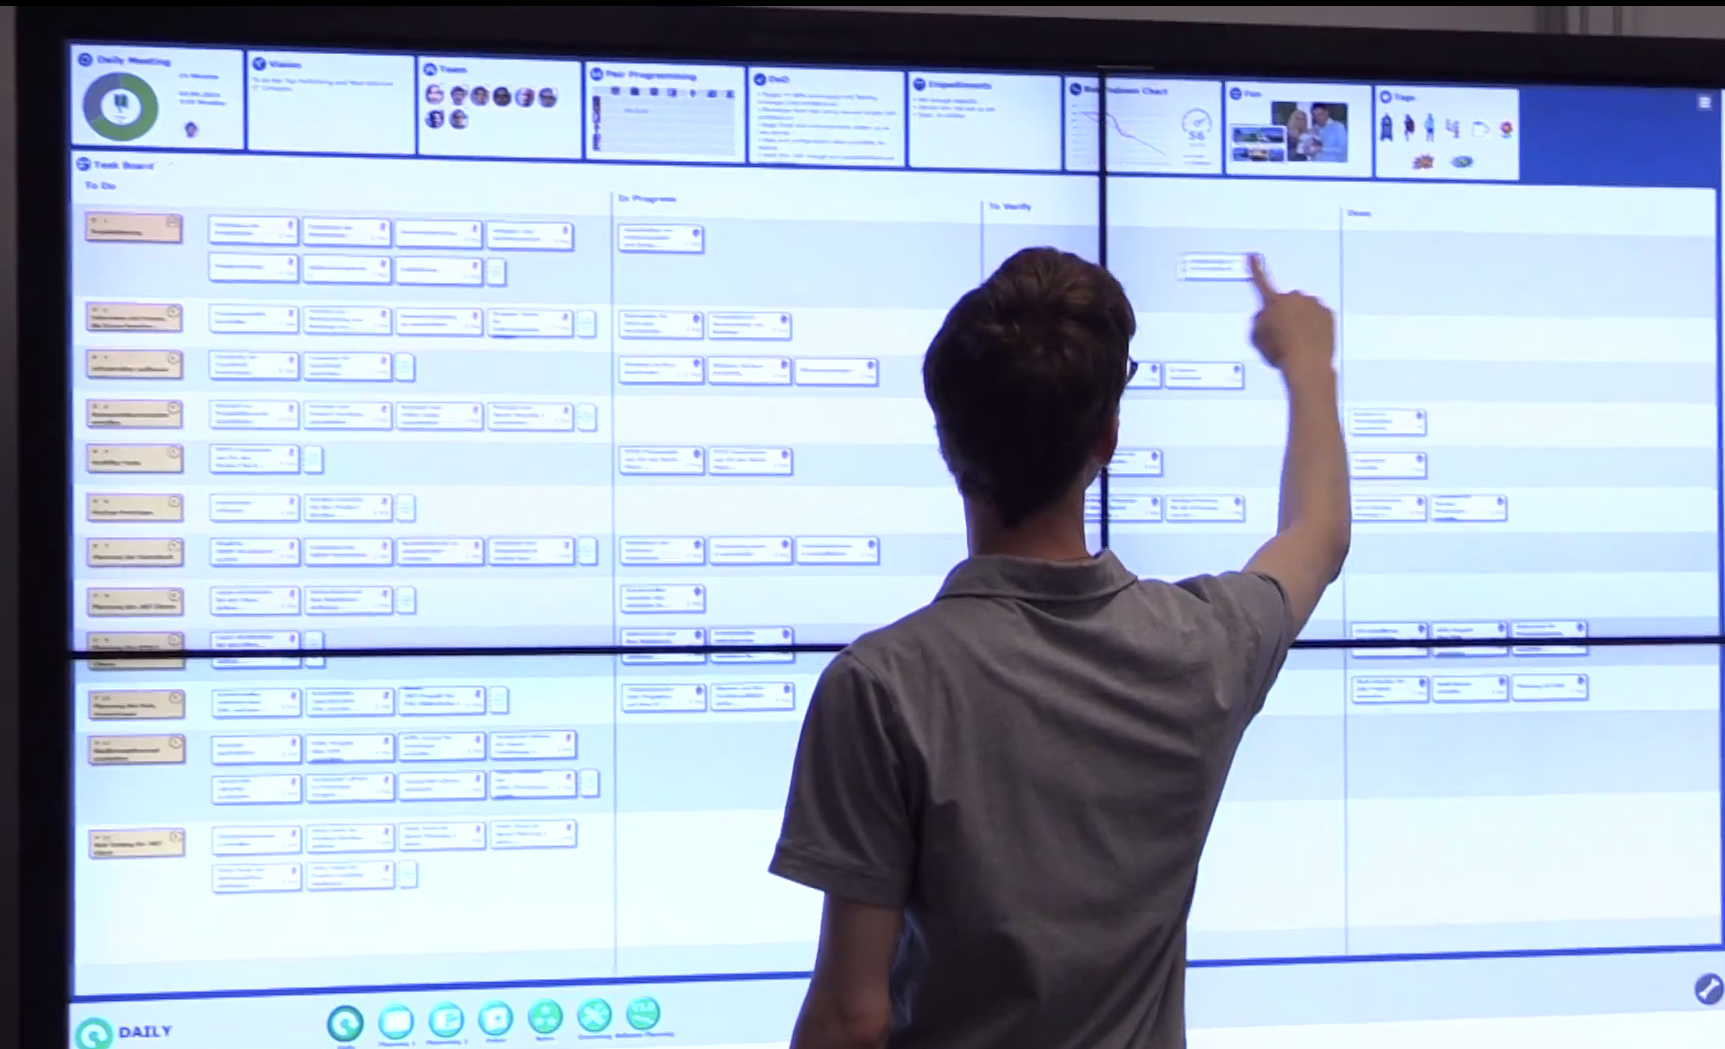
\includegraphics[width=\columnwidth]{figures/awall}
	\caption{The \textit{aWall} application running on a large multi-touch wall composed of 2x2 displays.}
	~\label{fig:awall}
\end{figure}

Using these two different interaction devices presents unique challenges regarding the interaction with the system as a team with the wall or as an individual with the tablet.

While a physical card wall offers many advantages with respect to ease of use and flexibility, it also has major disadvantages compared to digital solutions. However, recent studies \cite{udcw:31721, Mateescu:2015} show that current desktop-based digital solutions can hardly fulfill the requirements concerning agile collaboration.
Large digital multi-touch wall systems have the potential to be able to replace the physical boards and to offer even more possibilities, amongst are also support for distributed team collaboration. However as \cite{udcw:31721} and \cite{Mateescu:2015} show, they must provide the natural interaction and ease of use as physical boards. 

% - tablets for collaborative work
In \cite{Mateescu:2015} we present a concept for a large multi-touch wall based agile collaboration platform. The agile software development process comprises of different kinds of meetings, which can all be held at the wall. For some of the meetings a direct interaction with the wall, respectively with the artifacts represented at the wall, seem less appropriate. Other, smaller, input devices like individual developers tablets or even smartphones might be more appropriate. These devices allow multiple people to directly and independently interact with the artifacts on the wall and enter or modify data during the meeting more comfortable; still everybody immediately seeing the changes made. 


% What is SP2?
The user requirements for the software system are described in \textit{user stories}, a brief description of a feature in everyday language.
All \textit{user stories} are stored in a \textit{product backlog} and are maintained by a \textit{product owner}, who represents the customer to the development team and who is in charge of all requirements.
Each sprint starts with a \textit{sprint planning meeting}, which is divided in two sub meetings. In the \gls{sp1} meeting, the team and the product owner select those user stories, which will be implemented in the next iteration.
The selected user stories are stored in a list called the \textit{sprint backlog}.
In the \gls{sp2} meeting, the team then splits the selected user stories from the \textit{sprint backlog} into smaller technical tasks, which describe what the developer has to do to implement the user story. These tasks should not take longer than one workday to complete.


% - structure of the paper
The remainder of the paper is structured as follows.
First, related work is presented.
Then the UI design and the challenges we faced when adapting a web application designed for large screens to smaller tablet-sized screens.
In the next section, we present the architecture of the system we developed and how we tackled the challenges.
The following section describes the implementation and in the end, we discuss the work and provide an outlook into our future work.


\section{aWall Web Application}

\textit{aWall} is a web application developed for large multi-touch walls and for tablet sized computers.
The application offers several interaction possibilities, ranging from multiple people working on the wall simultaneously to people using the application with tablets and the wall together.
With the server of the system offering real-time updates to changes made with the application, all connected application-instances receive the modifications and are able to update the data in-place without reloading the website.

Figure~\ref{fig:awall} shows our setup using 2x2 full-HD monitors forming a 4K display.
Interactions can span monitors and are detected using an infra-red overlay in the frame around the four monitors.

It is based of configurable workspaces, that are composed of smaller widgets and one large main widget.
The main widget is always tailored to the a specific task that coincides with a meeting of the agile process.
The smaller widgets offer additional functionality and interaction possibilities.


\section{Related Work}
% Scrum taskboards stuff:
An often mentioned and typical setting used in the agile process is the taskboard.
It shows the current progress of the project iteration at a glance and is used in the daily stand-up meetings. 
A digital tabletop application is introduced for agile planning meetings in \cite{Ghanam:4599452}. 
The tabletop only has a single-touch display. 
Thus only one person can interact with the system at a time and without advanced gestures that involve multiple fingers like pinch-to-zoom.
In \cite{Rubart:2014:CMS:2669485.2669551}, a cooperative multi-touch taskboard for large displays is proposed. 
The paper discusses how interactive tabletops and surfaces can be applied to the agile taskboard for the daily stand-up and other meetings and evaluates gestures known from smartphones for big tabletops and group settings.
\cite{Haas:2014:TAV:2669485.2669538} introduces a task assignment system for tabletop computers that consists of two components: the tabletop application and a separate Android companion application.
The companion application shows changes made on the tabletop in real-time and offers some limited interaction capabilities.

% wall, tablet stuff
A multi-surface communication and collaboration platform using a wall, tabletops and tablets for an emergency operations center is presented in \cite{Chokshi:2014:EMM:2669485.2669520}. 
The system is spatially aware of all the devices and people in the room using multiple Kinects.
This allows the use of gestures like a flick on a tablet towards the wall to share information.
The device types are used for different scenarios:
The tablet is used for personal and private interaction with colleagues.
Whereas the tabletop is a semi-private workspace for collaboration and the wall is a public information radiator, aggregating multiple data sources.
The authors developed native applications for the wall, the tabletop and the tablet.
Thus multiple independent applications were developed with different code bases using in part the same information provided by servers.
% one web application to rule them (devices) all
With \textit{aWall}, we do not want to maintain multiple code bases but one application to handle all the devices.
This includes the viewing experience corresponding to the device type of what is shown and how it is presented.


% Responsive design:
One of the most significant challenges with the emergence of all the new devices like smartphones, tablets and phablets in the last years, is device and platform fragmentation.
Developing a unique experience for each device would mean to have an application per device type.
This also means multiple times the work if something needs to be changed. 
By using a single code base that serves a multitude of devices, a maintenance nightmare can be avoided.
For the web, HTML5 and CSS3 bring many advancements to create a single code base for different device and screen sizes.
The approach using a single application is called \gls{rwd}.
In \cite{Pandey:2013:RDT:2525194.2525271}, the author presents a case study of a mobile-first design process used to create a hybrid smartphone and tablet application for transaction banking.

% Proximity of user and responsive design:
What responsive design does not take into account is the proximity of the user. 
The authors in \cite{Sukale:2014:PWD:2638728.2638768} developed an example implementation of a responsive web application that adjusts the information displayed according to the user's distance to the display.

%Collaborative web visualization:
In \cite{Badam:2014:PCF:2669485.2669518}, an web-based application framework is presented for collaborative visualizations across multiple devices. The framework allows to synchronize UI state of new or legacy web applications with minimal overhead.


\section{UI Design and Challenges}

% traditional rwd:
% - normal sites: lots of content (pics and text)
% - we: mainly interaction
\todo{rwd: diff. between normal sites and aWall}

% tablet interactive to create stuff (normally not used for input)
% -not consume only
\todo{tablet is to create input, not only for consumption}

% collaborative aspect: see what's being created/ edited
\todo{collaborative aspect: see changes of others}

% difference to normal web apps
% how to bring all this information to tablet
\todo{howto bring to tablet}


\subsection{Responsive Design}
% - responsive web design
The \gls{rwd} \cite{Marcotte:2011} approach offers a solution to create one application that provides an optimal viewing experience across a wide variety of different devices with various display-resolutions. 
% - mobile-first, we: wall -> tablet "wall-first"
An important concept of \gls{rwd} is mobile-first \cite{Wroblewski:2011}. 
It is an approach to give the mobile site a higher priority and design it with the constraints and capabilities of small-screen devices in mind. 
The approach is based on the assumption that adding content to a website designed for small-screen devices is easier than removing content from the large desktop layout to fit the smaller screen.


% cornerstones of rwd
For the UI, the web application uses an approach called \gls{rwd} that builds on three cornerstones~\cite{Marcotte:2011}:
\begin{itemize}
	\item Relative units: The style and layout definitions should use relative units like percent instead of fixed units like pixel. A pixel is on a 1080p smartphone display does not have the same physical size as a pixel on a 1080p 24" desktop display. 
	
	\item Flexible images: The images are sized in relative units but there may also be multiple versions of the same image. For example, a low resolution image for small-screen devices and a higher resolution image for larger devices.
	
	\item Media Queries: Media queries are the main cornerstone of \gls{rwd}. They allow us to define breakpoints with conditional statements in the stylesheet at which different CSS style definitions take effect.
\end{itemize}

Media Queries have been introduced in CSS3 and became a W3C standard in June 2012 \cite{mediaqueriesW3C}.
They allow the content of a website to adapt to the conditions of the web browser.
The most prominent example of such a condition is the screen resolution.
By defining break-points, using for example the width of the viewport, the statement defines the style of the given \gls{dom} element.
% media query example
Let's assume we have a simple element with a title in a h1-element and a text in a p-element.
The media query could define that the p-element is hidden when the height of the viewport is less than 500 pixels.


\subsection{General Layout}
% context
The agile process has multiple collaborative meetings that deal with different aspects of the project.
% Workspace layout (info-view with widgets, workspace menu, main widget)
The UI of \textit{aWall} in Figure~\ref{fig:awall-layout} is built around workspaces configured with independent widgets that can be used by several workspaces.
For each meeting there is a workspace configured with the most appropriate widgets.
Each workspace consists of a main widget that takes most of the available space, numerous independent widgets in a panel at the top of the screen, called info-view, and the workspace-menu with options to configure the workspace.

\begin{figure}[h]
	\centering
	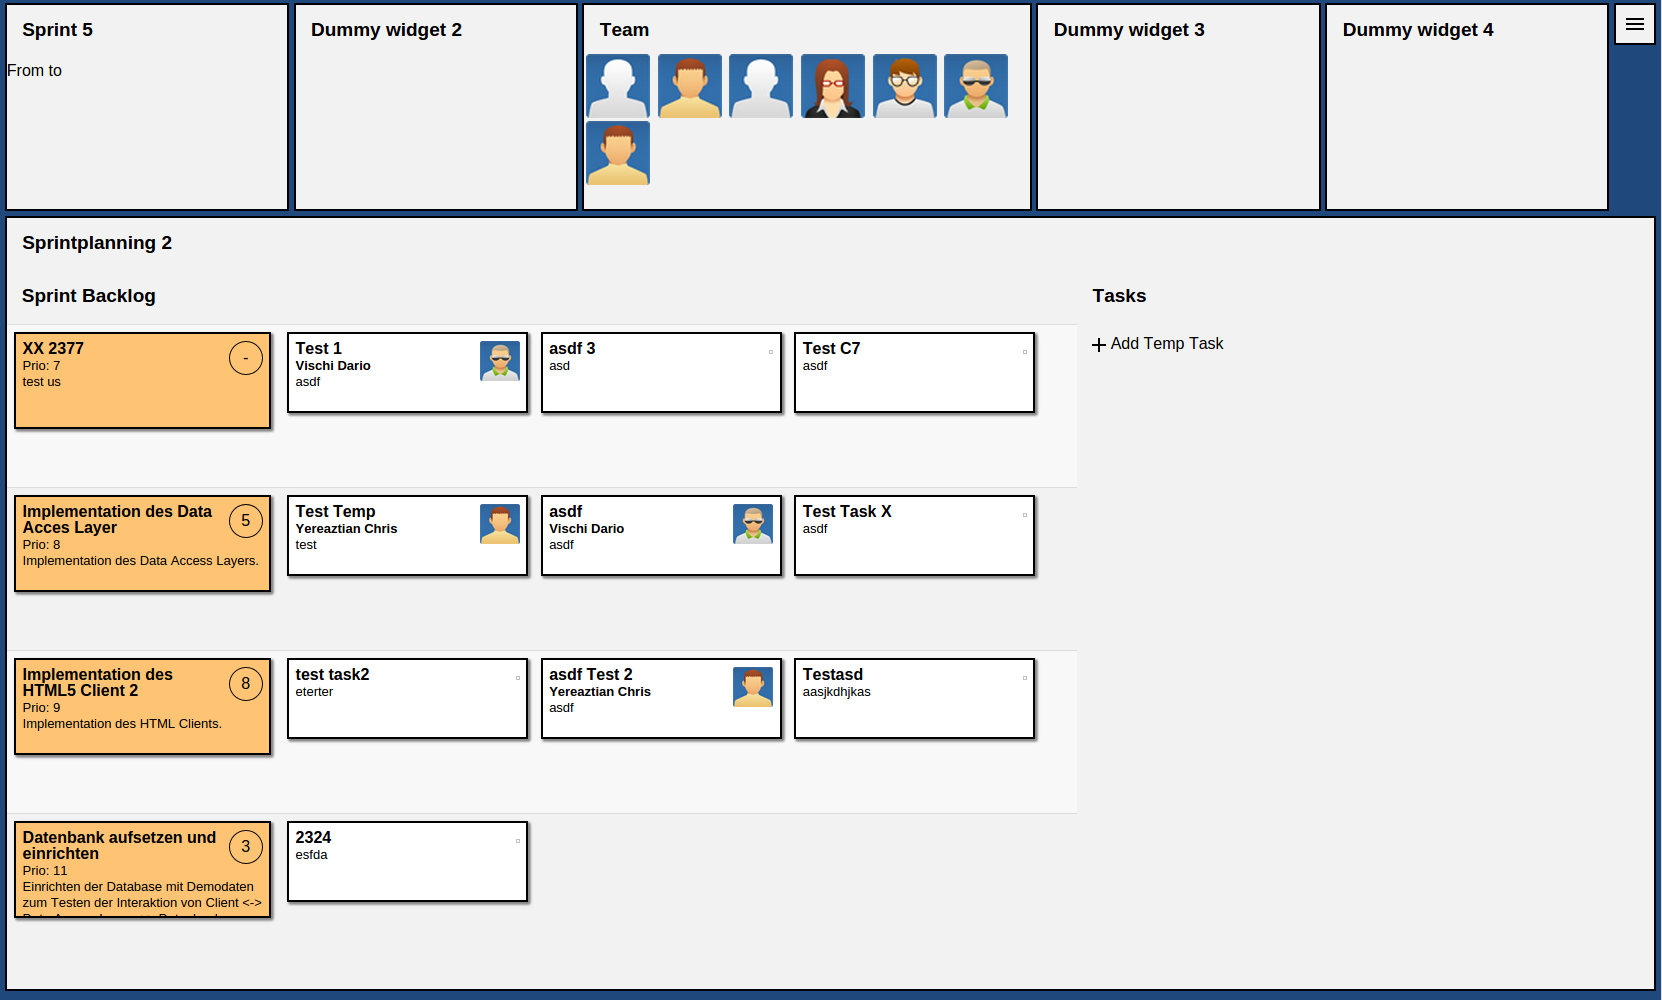
\includegraphics[width=\columnwidth]{figures/awall-layout}
	\caption{UI layout of \textit{aWall} with a main widget for \gls{sp2} as seen on the multi-touch wall.}~\label{fig:awall-layout}
\end{figure}

% main widget
The main widget occupies the largest part of the UI and is the main working area.
For each meeting of the agile process there is a specialized main widget that shows exactly what is needed and offers tailored interaction methods.
Supplemental interaction with additional artifacts is provided by the widgets in the info-view.
Each main widget is responsible for the responsive behavior of its content to show the appropriate amount of information depending on the available space.


% info view and widgets
The info-view is the horizontal panel at the top with the smaller widgets.
% responsiveness of number of widgets in the layout (min. width for widgets)
The widgets in the info-view can have different widths from standard width to multiple-times the standard-width.
The number of widgets to display is calculated by the application and depends on the width of the viewport.
If a currently hidden widget is enabled, the widget in the last position is replaced with the enabled widget.
This ensures that the widgets always have enough space.
Widgets that do not fit can be accessed by the workspace-menu, where each widget can be enabled or disabled. 


% widget abilities (dock, resize etc)
The widgets in Figure~\ref{fig:awall-layout} are in a docked position but can be undocked by dragging them out of the info-view.
When a widget is dragged out of the info-view (undocked) the space is closed whereby all widgets to the right move one position to the left.
If a widget is to be docked again, the widget's space is freed up with all widgets to the right moving one position to the right.
With this, the widgets can be freely arranged by the user.
Once undocked, the widget can be moved around the viewport and resized by either using the mouse or the pinch-to-zoom gesture on a multi-touch display. 



\begin{figure*}
	\centering
	\begin{subfigure}{0.4\columnwidth}
		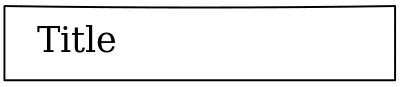
\includegraphics[width=\textwidth]{figures/widget-titleonly}
		\caption{}
		\label{fig:widget-titleonly}
	\end{subfigure}%
	\hfill
	\begin{subfigure}{0.4\columnwidth}
		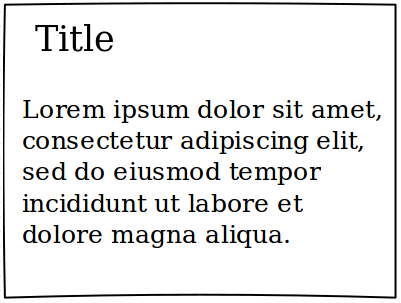
\includegraphics[width=\textwidth]{figures/widget-default-docked}
		\caption{}
		\label{fig:widget-default-docked}
	\end{subfigure}
	\hfill
	\begin{subfigure}{0.4\columnwidth}
		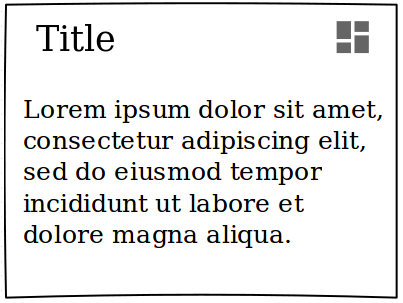
\includegraphics[width=\textwidth]{figures/widget-default-undocked}
		\caption{}
		\label{fig:widget-default-undocked}
	\end{subfigure}
	\hfill
	\begin{subfigure}{0.4\columnwidth}
		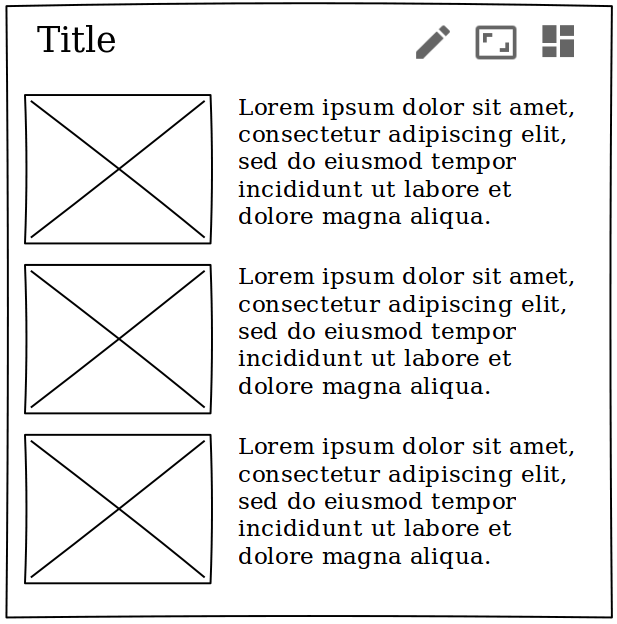
\includegraphics[width=\textwidth]{figures/widget-full}
		\caption{}
		\label{fig:widget-full}
	\end{subfigure}
	\hfill
	\begin{subfigure}{0.4\columnwidth}
		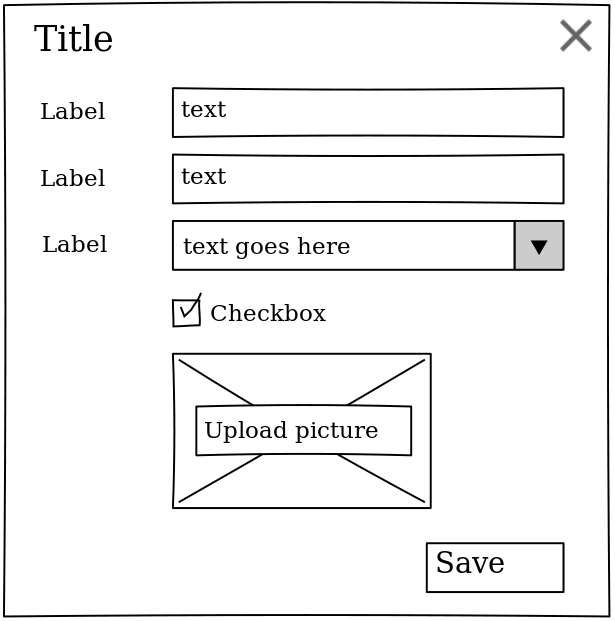
\includegraphics[width=\textwidth]{figures/widget-editmode}
		\caption{}
		\label{fig:widget-editmode}
	\end{subfigure}
	
	\caption{The different views for info-view widgets.}
	\label{fig:infoview-widgets}
\end{figure*}



% widgets sizes (title, default, full, edit mode)
The widgets can have multiple views for different sizes when being resized.
In the docked position in the info-view the widgets show the default view on larger screens. 
% responsiveness of the view (widget height with title only and default size)
On smaller screens like on a tablet, only the title of the widget is shown, henceforward called title-only view.
The default size with the same functionality as on larger screens is shown when it is undocked.
Besides the title-only and the default view, a widget can offer an additional full view and an edit mode.
The full view is intended to show more information on the widget's subject or offer additional interaction functionality.
It is triggered by specifying the breakpoints for the width and height.
Once the widget has exceeded both breakpoints while resizing, the full view is shown.
% - buttons when undocked (dock, reset size, enter edit mode)
If a widget has an edit mode, an edit icon is displayed in the top-right corner of the widget.
There are two more buttons on all widgets: one to reset the size to the default view and one that docks the widget in the info-view.


% workspace menu
% workspace menu: save/reset workspace, list of widgets with toggle to en/disable, list of available meeting workspaces
The workspace-menu is the small button in the top right corner.
It allows to control which widgets are enabled and disabled with toggles, to switch to other workspaces for the other meetings and to save or reset the current workspace configuration.
As mentioned above, the widgets in the info-view can be rearranged.
The new arrangement can be saved by the user or reset to the default.



\subsection{SP2 Layout}
The main widget for the \gls{sp2} meeting, as depicted in Figure~\ref{fig:awall-layout}, shows the \textit{sprint backlog} on the left and a panel on the right for unassigned tasks.
Unassigned tasks are specific to our solution and they represent the paper-based card written by a team member that has not been discussed by the team and thus has not been assigned to a user story yet.
This is where the tablets comes into play.
Each team member has a tablet and creates tasks with it.
As soon as the task is created on a tablet, it is sent to all devices connected to the system and pops up on the wall.
Then it is discussed and finally either assigned to a user story or discarded.

% responsiveness of sp2 workspace; 2 "views": large screen and small screen (sprint view: show all US, US view: show selected US and all tasks + temp tasks)
On the wall, everything including the \textit{sprint backlog} and the unassigned tasks can be shown simultaneously.
The tablet does not have enough space to show all the information like on the wall.
Thus we split the widget into two views:
The first view (Figure \ref{fig:sp2-overview}) shows all the user stories of the \textit{sprint backlog} in a grid.
When the user clicks, respectively selects a user story, the second view is shown, called detail view (Figure \ref{fig:sp2-detail}).
There the selected user story with all its tasks and the list of unassigned tasks is displayed.


\begin{figure*}
	\centering
	\begin{subfigure}[b]{1\columnwidth}
		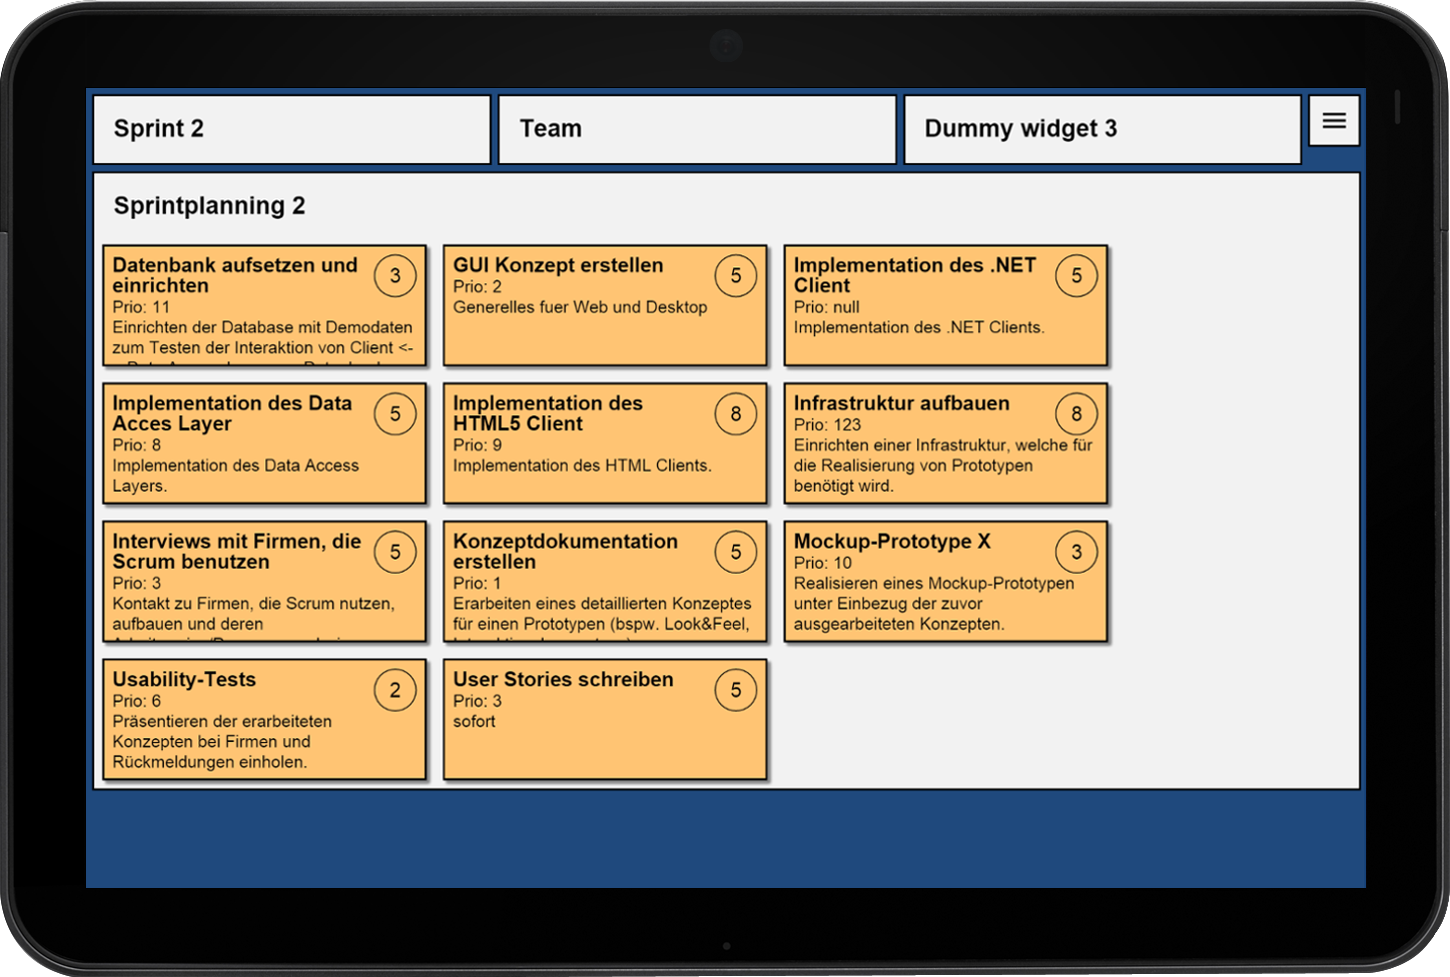
\includegraphics[width=\textwidth]{figures/sp2-overview-framed}
		\caption{Overview}
		\label{fig:sp2-overview}
	\end{subfigure}%
	\quad
	\begin{subfigure}[b]{1\columnwidth}
		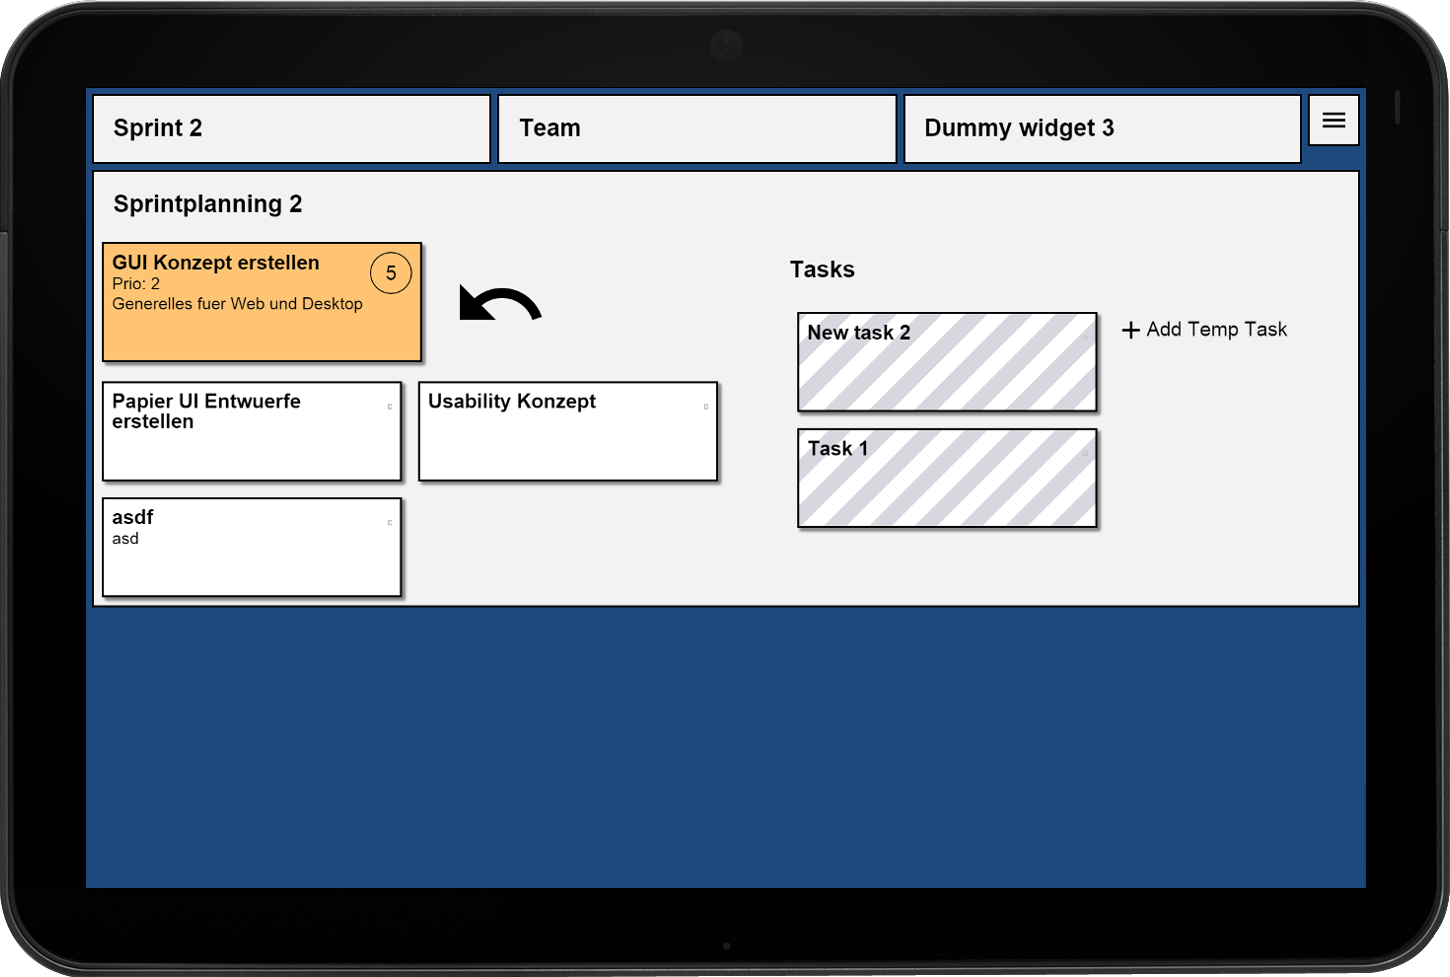
\includegraphics[width=\textwidth]{figures/sp2-detail-framed}
		\caption{Detailed view}
		\label{fig:sp2-detail}
	\end{subfigure}
	
	\caption{The two views of the split up \gls{sp2} user interface for smaller displays.}\label{fig:sp2-smallscreen-views}
\end{figure*}




\subsection{Challenges}

% see who is editing a task
% what happens when two people want to edit the same task
\todo{concurrent modifications}

% non UI challenge: platform independent 
\todo{platform independence}

The two device types the system uses, namely the wall and hand-held tablets, have significantly different screen resolutions and physical dimensions. 
An important goal driving our design was the ability to see everything without scrolling.
Supporting these different devices with one code base and adhere to the no scrolling requirement presents some challenges:

\begin{itemize}
	\item \textbf{Retain functionality:} 
	Even though the screen of a tablet is not as small as a smartphones', the available space is significantly smaller than on the large multi-touch wall. 
	A big challenge was to retain the same functionality on the tablet as on the wall. Often when going from a large screen to a smaller one, functionality is sacrificed in order to  keep it organized and legible.
	
	\item \textbf{Reduce space of non-essential elements:}
	% title-only view => undock => default view
	A lot of vertical space is used up by the info-view widgets.
	They offer auxiliary functionality, but it is not absolutely essential that they are completely visible the whole time in their default view.
	Thus, we created the title-only view for the widgets.
	That way, the widgets are still in the same place and visible, but have to be dragged out of the info-view to be usable.
	Once the widget is undocked, it enlarges to the default size and it can be used like on the wall.
	
	\item \textbf{Viewing experience: focused vs. overview:}
	In our collaborative scenario of the \gls{sp2} meeting, the wall and the tablet serve different needs.
	The wall's duty is to give the whole team the overview of the whole sprint, while the tablet's focus lies with the individual to create new tasks for the currently discussed user story.
	This requires the information displayed on the device to be specific to its purpose.
	While the complete \textit{sprint backlog} is important on the wall, it is not relevant for creating a task for a user story.
	Thus, we split the main widget for the \gls{sp2} meeting into two views on smaller screens as depicted in Figure \ref{fig:sp2-smallscreen-views}.
	
\end{itemize}



\section{Implementation}
%- Polymer, Interact.js
\subsection{Frameworks}
The \textit{aWall} web application uses Polymer~\cite{polymer}, a library that abstracts WebComponents and allows to define custom elements using declarative HTML tags instead of pure Javascript code.
This makes it easy to write new custom elements without the huge amount of boilerplate code that is required when using the native Javascript APIs directly.
For multi-touch gestures like pinch-to-zoom, drag\&drop and resizability of elements, \textit{aWall} uses the interact.js~\cite{interactJs} library.

\subsection{Responsive Widgets}
% how widgets are implemented by the developer developing widgets
All the widgets use the custom element \textit{awall-widget}.
It gives all the widgets the features like drag \& drop and resizability.
The four views of the widgets are also implemented by custom elements, namely \textit{awall-widget-title}, \textit{awall-widget-size-default}, \textit{awall-widget-size-full} and \textit{awall-widget-editable}.
Listing~\ref{lst:widget-elements} shows the pattern on how a widget is implemented using the aforementioned elements.
The title for a widget is given as the parameter to the attribute \textit{value} for the element \textit{awall-widget-title}.
For the other three view elements, the content is more comprehensive than just a string and thus is enclosed in the element's tags as indicated using HTML comment syntax.

\begin{code}[caption={HTML elements for the widget's different views.},label=lst:widget-elements]
<awall-widget>
  <awall-widget-title value="Team" />

  <awall-widget-size-default>
    <!-- Content for default view -->
  </awall-widget-size-default>

  <awall-widget-size-full showHeight="500" showWidth="400">
    <!-- Content for full view -->
  </awall-widget-size-full>

  <awall-widget-editable showHeight="500" showWidth="400">
    <!-- Content for edit mode -->
  </awall-widget-editable>
</awall-widget>
\end{code}

Not all the view elements must be used of course.
A widget does not need to have a full view or an edit mode.
Both are optional and can be configured using the two parameters \textit{showHeight} and \textit{showWidth} to define their breakpoints at which point they activate and the default view is hidden.
The edit mode is not shown automatically, but is represented by an edit button appearing when both breakpoints have been exceeded.


% how the custom element awall-widget is implemented by the framework
The \textit{awall-widget} custom element implements the features that all widgets have and controls when which view is displayed.
Listing~\ref{lst:awall-widget} depicts part of the template of the \textit{awall-widget} custom element.
The \textit{content} element is used in Shadow DOM and represents an insertion point for \gls{dom}-trees.
That means that everything between the start and end tag of \textit{awall-widget-size-default} in Listing~\ref{lst:widget-elements} is inserted in the position of the content tag that selects the \textit{awall-widget-size-default} in line 4 of Listing~\ref{lst:awall-widget}.


\begin{code}[caption={Part of the awall-widget custom element's template using insertion points for the different HTML tags.},label=lst:awall-widget]
<content select="awall-widget-title" />

<div id="extendedContent">
  <content select="awall-widget-size-default" />
  <content select="awall-widget-size-full" />
  <content select="awall-widget-editable" />
</div>
\end{code}


% visibility of the views
All elements in the template in Listing~\ref{lst:awall-widget} except \textit{awall-widget-title} are enclosed in an div-element whose visibility is controlled by the media query shown in Listing~\ref{lst:awall-widget-mediaquery}.
As long as the browsers viewport height is smaller than the defined \textit{max-height} breakpoint, only the title of the widget is shown.
When the widget is dragged out of the info-view, the default view becomes visible.
The widget can now be resized using the pinch-to-zoom gesture or the mouse.
During resizing, the width and height of the widget are compared to the \textit{showHeight} and \textit{showWidth} breakpoints defined for the full view and the edit mode.

\begin{code}[caption={Media Query hiding all the views except the title when the screen is small enough.},label=lst:awall-widget-mediaquery]
@media only screen and (max-height: 40rem) {
  #extendedContent {
    display: none;
  }
}
\end{code}

\subsection{SP2 Widget}
As mentioned before, each widget is responsible for its own responsive behavior.
The main widgets use the \textit{awall-widget} but with drag \& drop and resizability disabled.
The main widget for the \gls{sp2} workspace, as depicted in Listing~\ref{lst:sp2-template}, has two templates that are controlled by the boolean variable \textit{isSmallScreenHeight}.
The variable is set by the application's Javascript code and is accessible through Polymer's data binding mechanism.
Depending on the value of the variable one of the two inactive templates is activated.
The views are all compartmentalized into their own custom elements and thus the two templates in Listing~\ref{lst:sp2-template} only contain one element (results in Figure~\ref{fig:sp2-overview}) for the small-screen view and two elements for the large-screen view, that results in Figure~\ref{fig:awall-layout}.
The \textit{awall-userstory-cardlist} element for small screens handles its behavior to switch to the detailed view (Figure~\ref{fig:sp2-detail}) itself.
The title for the widget at the top of the listing is visible on any screen and thus is not enclosed in a template.

\begin{code}[caption={How the \gls{sp2} main widget decides which view to show.},label=lst:sp2-template]
<h2>Sprintplanning 2</h2>

<template if="{{isSmallScreenHeight}}">
  <awall-userstory-cardlist />
</template>

<template if="{{!isSmallScreenHeight}}">
  <awall-sprintbacklog />
  <awall-temptasks />
</template>
\end{code}


\section{Discussion}

\subsection{Hardware}
% 2x2 sucks because of the bezels when interaction requires the user to cross the bezel from one to another screen
\todo{bezel between the monitors in our setup}

% our 2x2 uses infrared to detect the touch points: when using pinch-to-zoom, the two fingers must have some distance between them or else only one touch-point is detected.
\todo{inaccurate touch-point tracking}


\subsection{UI Design}
% orientation of the tablet (portrait, landscape): only landscape supported atm
\todo{orientation changes on tablets}


% hand-writing with pen (test out and discuss)
\todo{handwriting}

% virtual keyboard overlays a lot of space and hides the application
\todo{virtual keyboard hiding content}



\subsection{Responsive Design}
% use of RWD (ad/disadvantages) in aWall
In combination with new best practices like \gls{rwd}, enabled by the new standards, the development of new and adaptable web applications becomes more approachable.
Especially media queries allow us to detect and react to changes of factors like the screen resolution that are important for the rendering of content.
They allow us to either hide elements or render them using a different style (e.g. smaller font).
Together with the HTML template element, that allows to create inactive \gls{dom}-trees, conditional templates can be defined that are shown depending on a boolean variable set by a media query.

% the two views of SP2 for small-screen devices
The main widget for the \gls{sp2} workspace presented in this paper uses such conditional templates to present its content depending on the size of the browsers viewport dimensions.
The views including their specific behavior for both display sizes we implemented, namely the large wall and the tablet, have to be developed separately.
Thanks to the use of custom elements even for the REST API, the separate views only have to include a HTML element in their HTML code to access it.
The data is then available in the whole element using data binding provided by Polymer.


\subsection{Implementation}
The framework we developed with \textit{aWall} shows, that current web technologies and emerging new web standards make it possible to build an application that serves different devices with disparate screen resolutions and physical size using a single code base. 

% use of WebComponents (advantages)
Through its design of using loosely-coupled web components, specifically custom elements with Shadow DOM, there are no dependencies between the widgets.
This allows a developer to create new widgets without worrying about whether there are going to be problems with other widgets like  giving an element an ID that has already been used or having its stylesheet definitions (CSS) affect other elements of other widgets.

% WebComponents: rapid development (0.5 -> 1.0), many changes
By working with the newest technologies, there is always the problem with rapidly evolving and changing APIs and libraries.
Since we started to develop \textit{aWall}, the Polymer library evolved and reached version 1.0 with lots of changes.
It is going to take some time to port the current application to the new version. 

% WebComponents only work natively with Chrome, polyfills for other browsers
Another inconvenience of using the newest web technologies is that the number of browsers implementing all those new features is limited.
Currently, \textit{aWall} only runs natively on the Chrome and Chromium web browsers.
Most other browsers are in progress of implementing the specifications for web components.
For all those browsers not supporting any or all the features, there are so called polyfills available.
Polyfills are Javascript libraries, that add the missing APIs to the browser.
One big disadvantage of using polyfills is their lower performance compared to the native implementations.


\section{Conclusion and Future Work}
% conclusion
In this paper we presented how we designed and developed a responsive web application using a single code base that provides the appropriate viewing experience on the large wall as well as the much smaller screen of a tablet without sacrificing functionality.
As an example, we used the \gls{sp2} meeting of the agile process, where multiple people create tasks for a user story which are then discussed together on the wall, to showcase the responsive and collaborative nature of \textit{aWall}.

%results from taskboard UI tests (-> tasks for future work)?
After the design of the large-screen UI, we conducted some live-action interviews with developers to discover if the wall could be something they want to work with and to get input on how to improve it.
%meetings with a distributed team (e.g. show movement when a task is dragged) [similar to PolyChrome]
In the future, we are going to build on the input we received and would also like to extend the wall to work with distributed teams, where the movement of a task for instance is mirrored on other walls.


\balance{}

% REFERENCES FORMAT
% References must be the same font size as other body text.
\bibliographystyle{SIGCHI-Reference-Format}
\bibliography{references}

\end{document}

%%% Local Variables:
%%% mode: latex
%%% TeX-master: t
%%% End: